\documentclass[aps,prl,twocolumn,groupedaddress]{revtex4-1}
\usepackage{graphicx}
\usepackage{amsmath}

\begin{document}
\title{Optical Pumping and Magnetic Resonance}
\author{Dongwon Han}
\author{Kevin Wood}
%\email[]{kevin.wood@stonybrook.edu}
%\thanks{}
\affiliation{Stony Brook University}

\date{\today}

\begin{abstract}
% insert abstract here
\end{abstract}

\maketitle

% body of paper here - Use proper section commands
% References should be done using the \cite, \ref, and \label commands
\section{Introduction}
%%%%%%%%%%%%%%%%%%%%%%%%%%%%%%%%%%%%%%%%
%%%%%%% Kevin is working on this %%%%%%%
%%%%%%%%%%%%%%%%%%%%%%%%%%%%%%%%%%%%%%%%
Rubidium (Rb) is an alkali metal with atomic number $Z=37$.
Neutral states contain four entirely filled electron shells with no net angular momentum and a single valence electron.
In its ground state, the valence electron carries no orbital angular momentum: $5^{2}S_{1/2}$.
In its first exited state, the valence electron carries one quanta of orbital angular momentum which can either align or anti-align with its spin contribution: $5^{2}P_{1/2}$ or $5^{2}P_{3/2}$. %"align or anti-align" probably isn't the best way to say this...

The energy splitting of the $5^{2}S$ and $5^{2}P$ states due to the Coulomb interaction with the nucleus is on the order of a few electron-volts.
The degeneracy of the first excited state is lifted by the spin-orbit coupling in which the electron's spin couples to the magnetic field set up by the positively charged nucleus in motion relative to the electron.
This effect introduces an energy gap is on the order of $10^{-2}$ electron-volts between the $5^{2}P_{1/2}$ and $5^{2}P_{3/2}$ states.
A similar interaction between the nucleus and the magnetic field set up by the electron causes further energy splitting which are on the order of $10^{-9}$ electron-volts, and it is this interaction that we will be probing by applying the techniques of optical pumping and magnetic resonance.

%overview of optical pumping

%overview of magnetic resonance

\section{Review of Previous Work}
\section{Experimental Set-up}

%%%%%%% DW is working on this %%%%%%%
The entire apparatus is titled such that the center line of the apparatus is roughly parallel to the magnetic field of the Earth. The schematic of experimental design is shown in figure \ref{exp_schematic}.
\begin{figure}
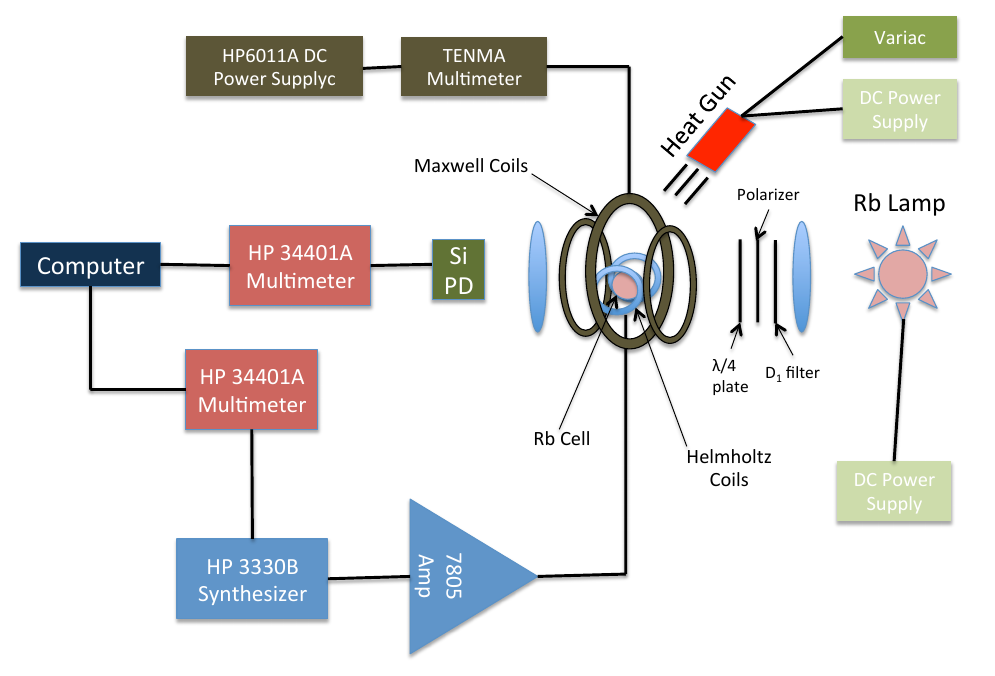
\includegraphics[width=\columnwidth]{exp_setup_schematic.png}
\caption{\label{exp_schematic}  Schematic of experimental setup}
\end{figure}

We use the Rb discharge lamp and a lens to produce collimated Rb $D_1$ and $D_2$ lines.
We select circularly polarized D1 light by applying a spectral filter and a linear polarizer with quarter wave plate. The filtered light is directed to a heated Rb Cell, which contains both $Rb^{85}$ and $Rb^{87}$ isotopes. The Rb cell also contains Argon as a buffer gas. By preventing the Rb atoms hitting the wall too frequently, the buffer gas slows down the depolarization process. The light emerges from the cell is refocused into a Si photodiode, which converts light to current. The signal from the photodiode is amplified before recorded by LabView software. We use LabView software to collect and store collected signal. 

We use Maxwell coils to produce a uniform magnetic field around the Rb cell. The Maxwell coils are arranged in the three coil configuration originally designed by James Clark-Maxwell in 1873. This configuration enables us to convert DC current to a homogeneous magnetic field of known intensity. This device is consisted of two smaller coils (labeled A and C) and one larger coil (labeled B). The two smaller coils A and B are symmetrically placed with respect to coil B. The displacement between the center of coil B and the center of smaller coil is $26.5\pm0.2$cm. 

The coils are wound with copper wire of the diameter $0.132\pm0.005$cm. The numbers of layers and turns per each layer is summarized in the table \ref{maxcoil}. The inner diameter of Coil B is $78.4\pm0.5$cm. Two smaller coils A and C has the inner diameter of $59.1\pm0.5$cm. The Maxwell coils are shown in Figure \ref{exp_photo}. 

\begin{figure}
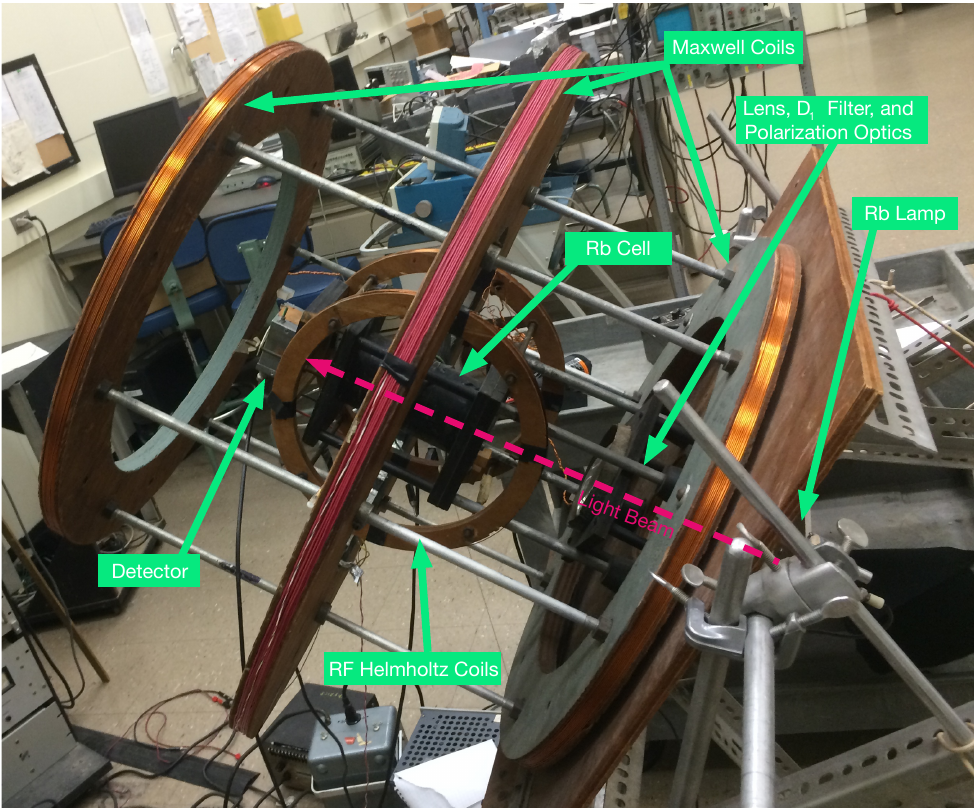
\includegraphics[width=\columnwidth]{exp_setup_photo.png}
\caption{\label{exp_photo} The optical pumping experiment apparatus}
\end{figure}

\begin{table}
\centering
\begin{tabular}{|c|ccc|}
\hline
Layer \#  & Coil A & Coil B & Coil C \\
\hline
1 & 11 & 11 & 11 \\
2 & 10 & 10 & 10 \\
3 & 11 & 11 & 11 \\
4 & 10 & 10 & 10 \\
5 & 11 & 11 & 11 \\
6 & 10 & 10 & 10 \\
7 & 11 & 11 & 11 \\
8 & 10 & 10 & 11 \\
9 & 11 & 11 & 11 \\
10 & 10 & 10 & 11 \\
11 & 5 & 11 & 3 \\
12 & 0 & 10 & 0 \\
13 & 0 & 11 & 0 \\
14 & 0 & 5 & 0 \\
\hline
\end{tabular}
\caption{\label{maxcoil} Number of layers and turns per each layer of three Maxwell coils}
\end{table}

A set of Helmholtz coil is placed orthogonal to the three Maxwell coils around the Rb cell. These second set of coils are used to generate Radio Frequency (RF) field, which is controlled by a synthesizer. We use the synthesizer to sweep various RF frequencies to locate the resonance frequencies of $Rb^{85}$ and $Rb^{87}$ isotopes. 

\section{Theoretical Model}
%%%%%%%%%%%%%%%%%%%%%%%%%%%%%%%%%%%%%%%%
%%%%%%% DW is working on this    %%%%%%%
%%%%%%%%%%%%%%%%%%%%%%%%%%%%%%%%%%%%%%%%

We first consider an atom with atomic number $Z$ orbited by $Z$ bound electrons. To the
leading order, its interaction is described by Coulomb potential between atomic nucleus and electrons and between electrons. Since the mass of the nucleus $M$ is much greater than that of electron $m_{e}$, i.e. $M \gg m_{e}$, we can use Born-Oppenheimer (BO) approximation to separate the motion of atomic nucleus and bound electrons. In the rest frame of the nucleus, the following Hamiltonian describes the leading order interaction.    

\small\begin{equation}\label{eq:leading_h}
\hat{H}_0 = \sum_{n=i}^Z \bigg(\frac{-\hbar^{2}}{2m_{e}}\nabla^{2}_{i} - \frac{1}{4\pi\epsilon_{0}}\frac{Ze^{2}}{r_{i}}\bigg) + \sum_{pairs ij}\frac{1}{4\pi\epsilon_{0}}\frac{e^{2}}{|r_{i}-r_{j}|} 
\end{equation}

Because the Coulomb interaction between electrons, the third term in the equation \ref{eq:leading_h}, is nonlinear, we cannot find a analytic solution to this Hamiltonian except few special cases. Hydrogen like atom, which one studies in elementary quantum mechanics, is such special case. For Hydrogen like atom, the solution to the equation $\hat{H}_0$ and the corresponding energy are given by.

\begin{equation}\label{eq:hatom_sol}
\psi_{nlm}(r,\theta,\phi) = R_{nl}(r)Y^{m}_{l}(\theta, \phi) 
\end{equation}

\begin{equation}\label{eq:hatom_e}
E_{n} = \frac{-m_{e}c^{2}\alpha^{2}Z^{2}}{2n^{2}}
\end{equation}

Where $\alpha$ is the fine structure constant, and $n$, $l$, and $m$ are quantum numbers.
To the leading order, the energy level of a Hydrogen like atom is solely determined by its principal quantum number n. % This is only true to first order, right? m and l matters for the fine structure energy splitting.. 
The other two quantum numbers l and m determine the total angular momentum and the angular momentum component along z-axis respectively. 

We can use solution to Hydrogen like atom and its energy levels as a framework to describe more complex atoms like Rubidium. The Paul Exclusion principle states that two identical fermions cannot occupy the same quantum state. This allows us to "build up" multi-electron wave-functions by placing electrons into the lowest available energy level one by one. This idea is summarized in the Aufbau principle, which states that electrons orbiting atomic or molecular nucleus fill the lowest energy levels before filling the higher levels. In this experiment, we use Rubidium atom which have 37 electrons with the ground state configuration $1s^{2}2s^{2}2p^{6}3s^{2}3p^{6}3d^{10}4s^{2}4p^{6}5s^{1}$ 
%\footnote{for more details about notation, please see https://en.wikipedia.org/wiki/Electron_configuration}.
Core electrons of Rubidium, those with principal quantum number $n \l 5$, are "invisible" to our spectroscopy. Hence, we can simplify our analysis by only considering single valence electron.

So far, our model has taken account of only Coulomb interaction between various components of a atom. The energy level of this model is degenerate. 
If we want to break the degeneracy, we need to take account of relativistic corrections in our Hamiltonian. 
In the week magnetic field limit, under which this experiment is performed, the next order correction is spin-orbit coupling.
Spin-orbit coupling is due to the interaction between the spin of a electron and the magnetic field generated by the orbit of electron. 
In this experiment, the spin orbit coupling breaks $5P$ energy level degeneracy by splitting it into $5^2P_{1/2}$ and $5^2P_{3/2}$. 
Spin-orbit coupling effect is about 9 orders of magnitude smaller than  Coulomb interaction. 

\begin{figure}
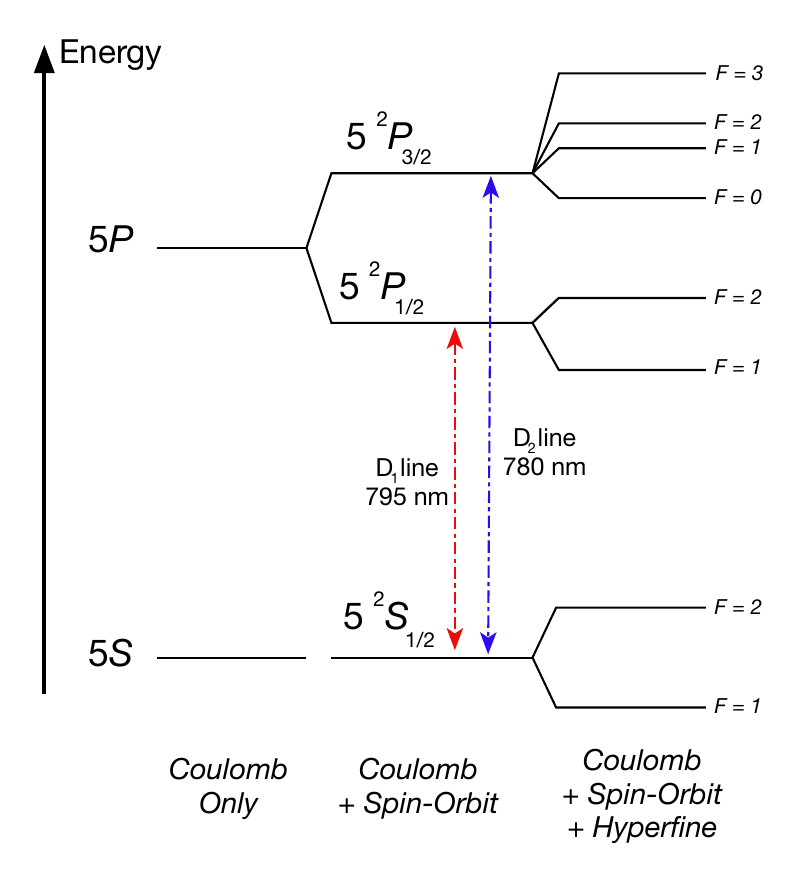
\includegraphics[width=\columnwidth]{Rb87_elevel_ver2.png}
\caption{\label{rb87_elevel} Schematic diagram of the energy level splitting of $^{87}Rb$}
\end{figure}

\subsection{Hyperfine Splitting}% for magnetic resonance explanation
The next order correction to our Hamiltonian is called Hyperfine Splitting, which is due to the interaction of nuclear spin and magnetic field. 

\section{Measurements}
%%%%%%%%%%%%%%%%%%%%%%%%%%%%%%%%%%%%%%%%
%%%%%%% Kevin is working on this %%%%%%%
%%%%%%%%%%%%%%%%%%%%%%%%%%%%%%%%%%%%%%%%
The optical pumping and magnetic resonance technique allows for a rich suite of measurements to probe the detailed atomic structure of relatively complicated elements.
Here we present measurements of the absorption cross-section of (optically pumped) Rubidium gas, the magnetic moments of the $^{85}\text{Rb}$ and $^{87}\text{Rb}$ isotopes, and hyperfine splitting.
\subsection{Rb Absorption Cross Section}

The absorption cross section of Rubidium was measured as the Rb cell warmed through the application of the Beer-Lambert law, which predicts the following relationship between the transmitted intensity of light and the number density of Rb atoms:
\begin{equation}
I=I_{0}e^{-\sigma nl}.
\end{equation}
Here $I$ is the transmitted intensity, $I_{0}$ is the intensity of the incident light, $n$ is the number density of Rb atoms, and $l=0.05\text{ m}$ is the cell length.
The transmittance for a given Rb density was recorded via the photodiode, and the temperature of the cell was measured crudely with a mercury thermometer for each reading.
The monatomic Rubidium gas inside the cell is well-described by the ideal gas law
\begin{equation}\label{eq:idealgas}
n=\frac{N}{V}=\frac{P(T)}{k_{b}T}.
\end{equation}
At constant volume, the pressure of Rubidium gas as a function of temperature has been parameterized as the following:
\begin{equation}\label{eq:PofT}
P(T)=10^{4.857-4215/T}\text{ atm}
\end{equation}
where temperature $T$ is given in units of Kelvin.
Putting together Equations \ref{eq:idealgas} and \ref{eq:PofT} allows the determination of the Rb number density from the temperature measurements:
\begin{align}
n&=\left(\frac{101325.0\text{ Pa}}{1\text{ atm}}\right)\frac{(10^{4.857-4215/T}\text{ atm})}{(1.38\times10^{-23}\text{J/K})T}\\
&=1.006\times10^{33}\left(\frac{10^{-4214/T}}{T}\right)\text{ m$^{-3}$}
\end{align}
Figure \ref{RbXsection} shows the data from which we calculate value of the cross-section to be
\begin{equation}
\sigma=(6.06\pm0.06)\times10^{-17}\text{ m$^{-3}$}.
\end{equation}

\begin{figure}
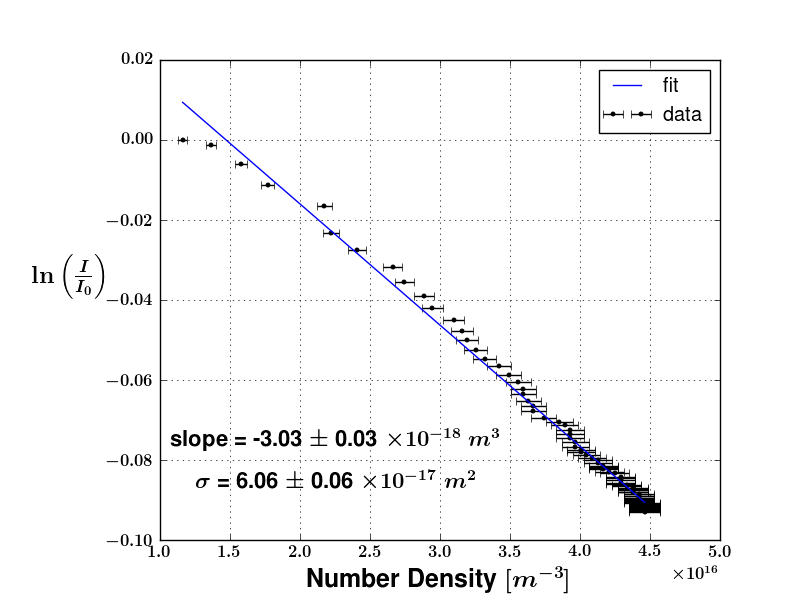
\includegraphics[width=\columnwidth]{rb-absorption-xsection.png}
\caption{\label{RbXsection} The absorption cross section of Rubidium  from the application of Beer-Lambert�s law to data taken as the Rb cell warmed.}
\end{figure}

\subsection{$^{85}$Rb and $^{87}$Rb Magnetic Moment}

By introducing an alternating magnetic field at a frequency corresponding to the energy splitting between 

\begin{figure}
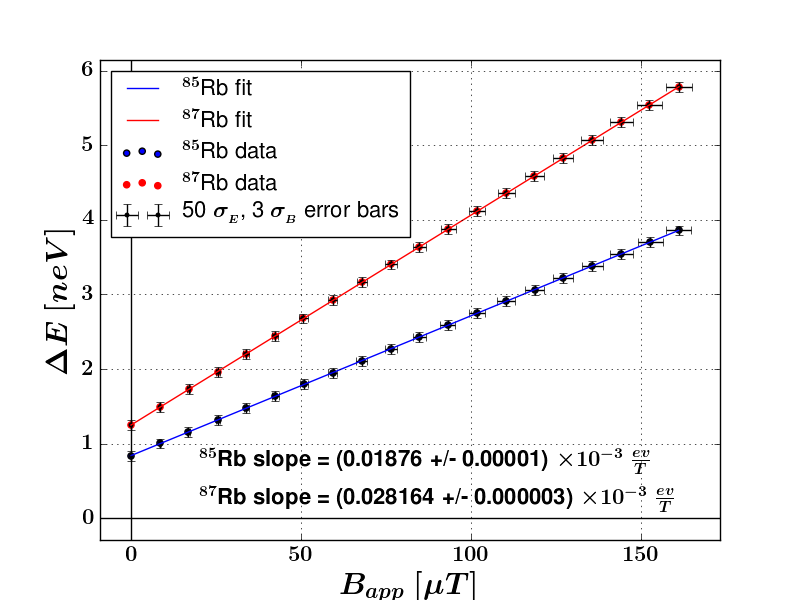
\includegraphics[width=\columnwidth]{magmom.png}
\caption{\label{MagMom} Measurement of the magnetic moment of $^{85}$Rb and $^{87}$Rb.}
\end{figure}

\subsection{Hyperfine Splitting}

\begin{figure}
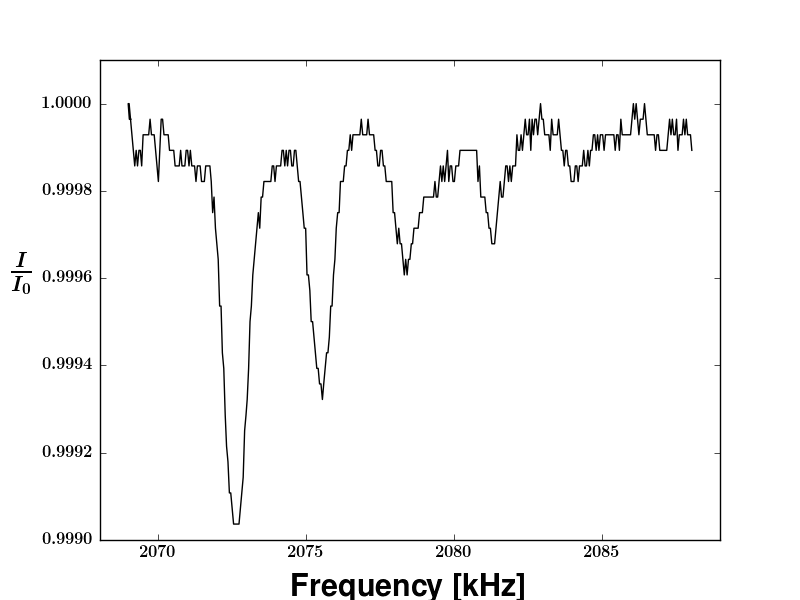
\includegraphics[width=\columnwidth]{rb85-hyperfine_split.png}
\caption{\label{HyperFineSplit} (data) Observation of hyperfine splitting of $^{85}$Rb.}
\end{figure}

\section{Comparison of Data and Theoretical Model}
%%%%%%%%%%%%%%%%%%%%%%%%%%%%%%%%%%%%%%%%
%%%%%%% Kevin is working on this %%%%%%%
%%%%%%%%%%%%%%%%%%%%%%%%%%%%%%%%%%%%%%%%
\section{Discussion and Conclusions}
\section{Author Contributions}

%Kevin: data analysis, "introduction", "measurements", "comparison of data and theoretical model",
%DW: data acquisition, "experimental set-up", "theoretical model"

%unclaimed: "Review of previous work", "discussion and conclusions"

\bibliography{basename of .bib file}

\end{document}